\chapter{Literature Review} \label{ch:litreview}
This chapter brings together constellation design, uncertainty-aware optimization, orbital-debris remediation, and the transfer theory needed to connect them. Each literature contributes a bounded piece of the problem. Walker's structured-shell formulations \cite{walker1970,walker1984}, Mortari's Flower-constellation framework \cite{mortari2004,mortari2006acta,ruggieri2006flower}, search-based constellation studies such as Williams et al.\ \cite{williams2001MOGA} and Ferringer and Spencer \cite{ferringer2006jsr}, and recent uncertainty-aware mission-design work \cite{GondelachLinares2019,EddyKochenderfer2019,NormanRivest2024} establish adjacent foundations. Remediation and conjunction-assessment studies establish intervention mechanisms and probabilistic risk logic \cite{JARRY2019185,Phipps2011lodr,GonzaloColombo2020,RyuBouvierLalani2024}. The narrow gap addressed here is their operational integration: a catalogue-conditioned natural conjunction bank, short-horizon dust-enabled \gls{jca} transfer and uncertainty evaluation, and deployer-architecture comparison under explicit reliability and resource semantics. This is an integration claim, not a claim that any individual component is new.

\begin{figure}[htb]
    \centering
    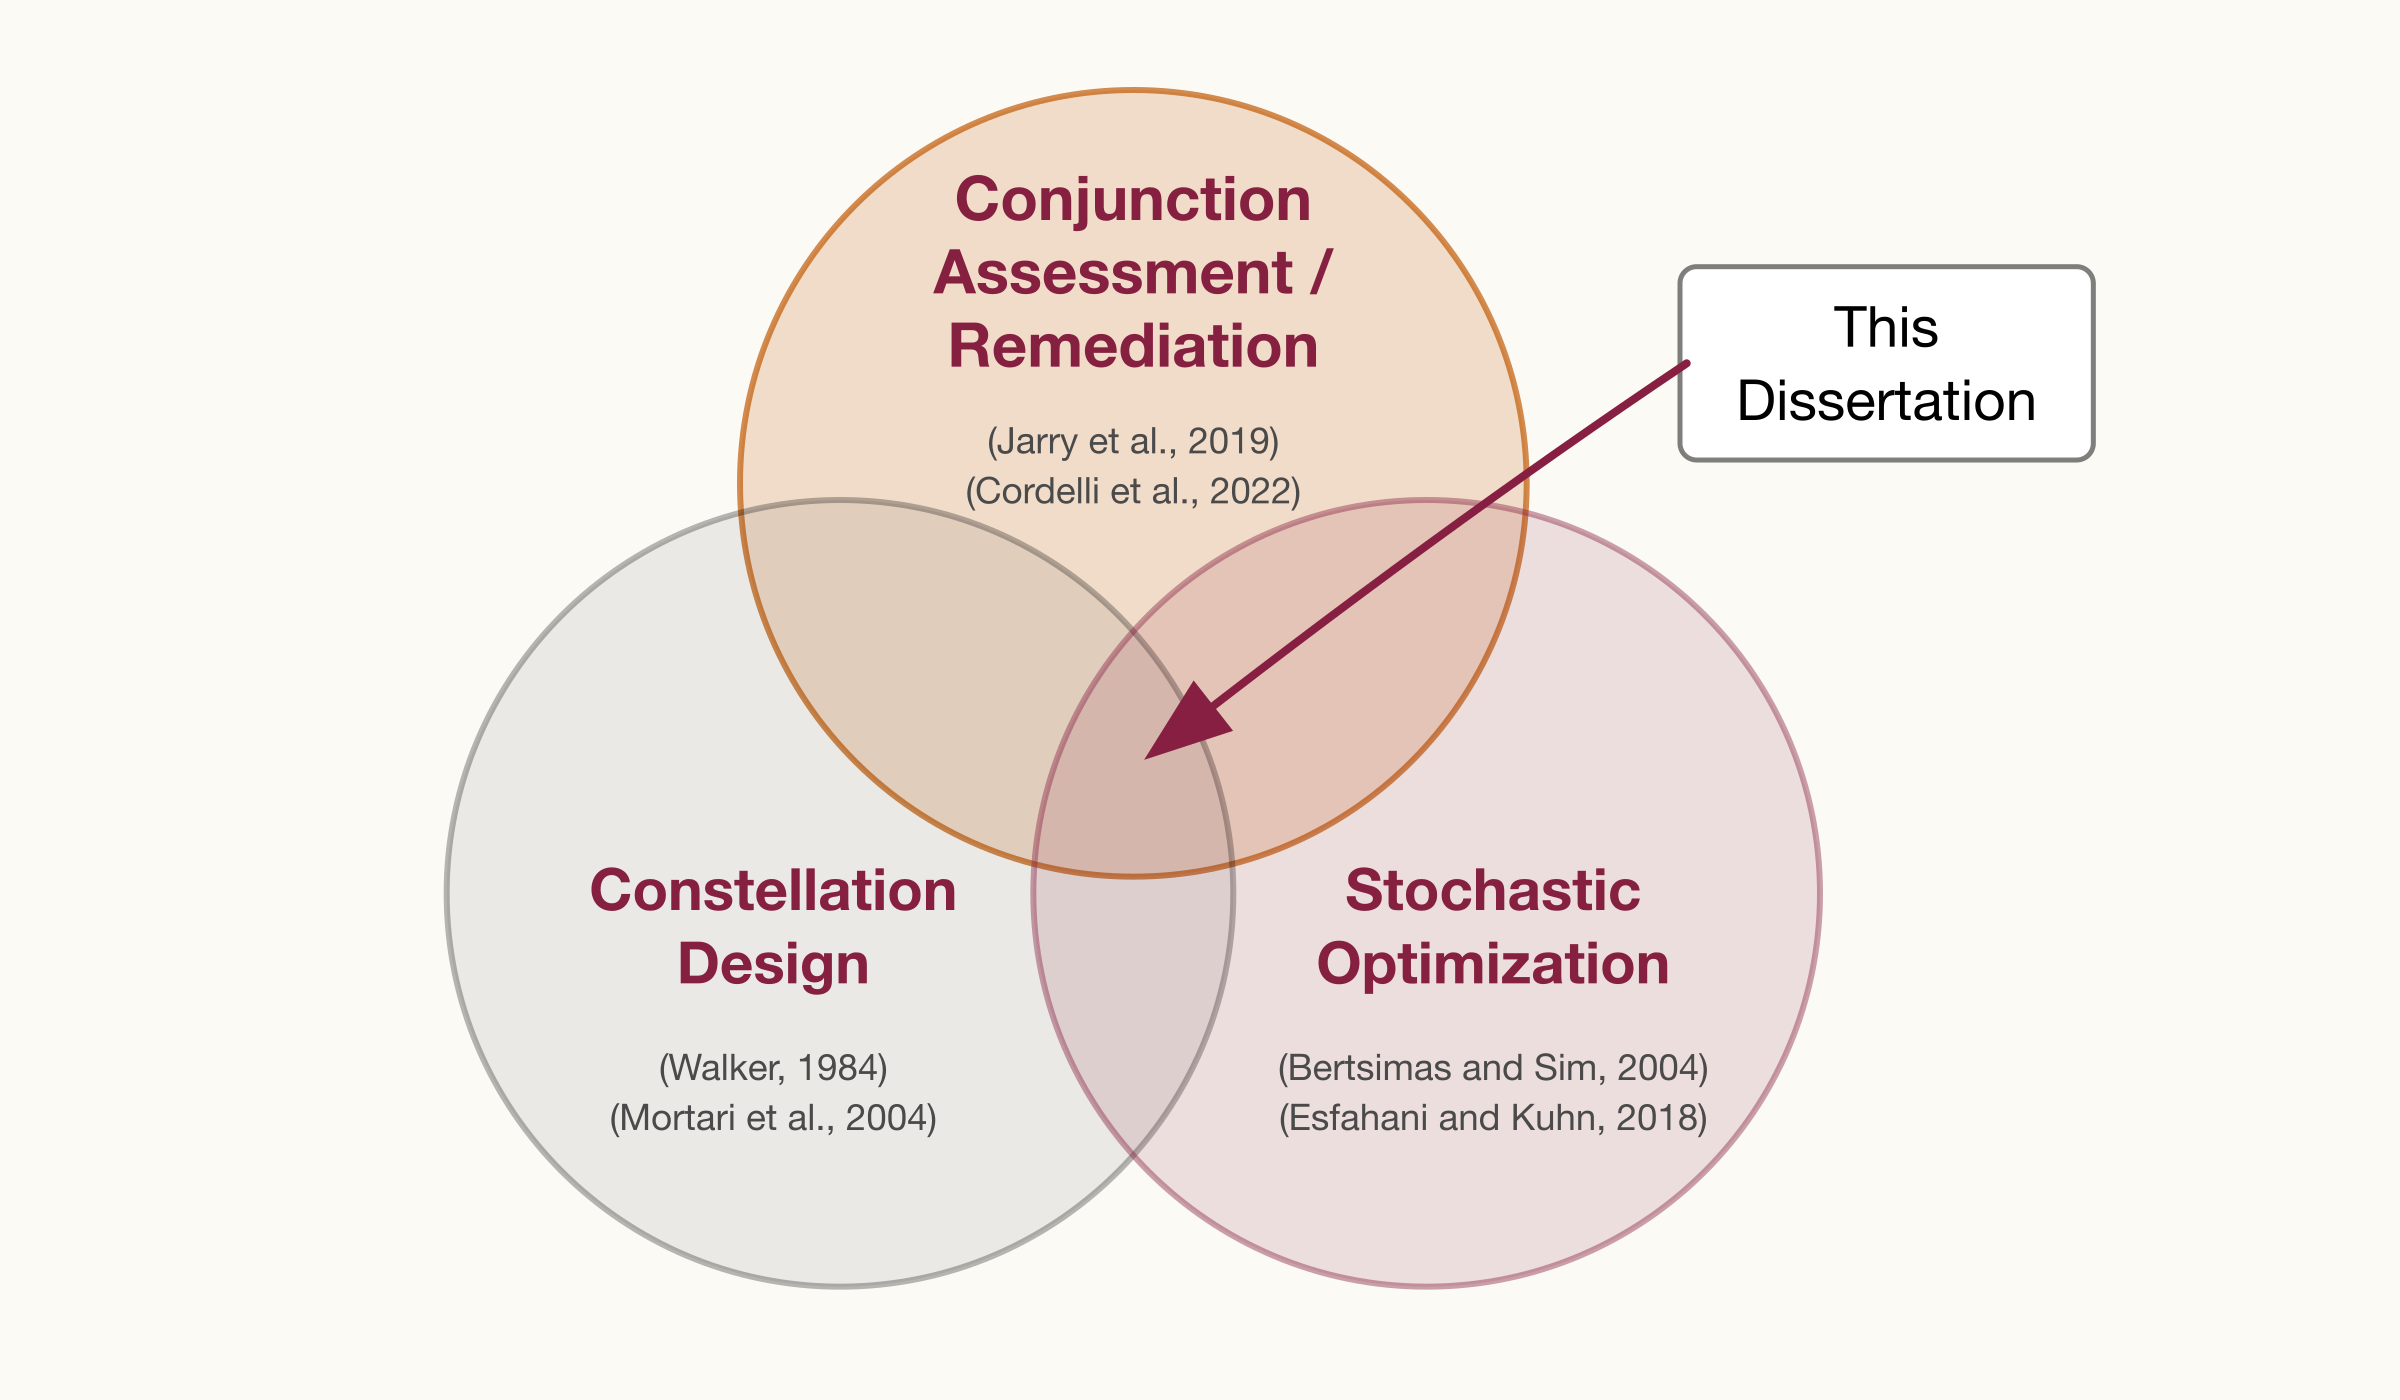
\includegraphics[width=0.84\linewidth]{figs/sota_venn.png}
    \caption[State-of-the-art synthesis]{High-level synthesis of the study's literature position. Constellation design, remediation or collision-avoidance interventions, and uncertainty-aware optimization are all established research areas; this work addresses the gap at their intersection by treating hazardous-event evidence, event-level physics, and architecture search as one integrated design problem.}
    \label{fig:sota_venn}
\end{figure}

\section{Constellation Optimization} \label{se:consteloptim}
Constellation design is usually approached from two complementary directions. One is geometric and analytic: structured families are studied because their symmetry yields interpretable coverage, revisit, and maintenance behavior. The other is algorithmic: the constellation is treated as a design vector and searched against one or more mission objectives. Both perspectives matter here because deployer constellations must remain physically interpretable while still being flexible enough to react to a highly anisotropic debris environment. For this dissertation, the useful question is what each family or optimizer adds to the design freedom needed for a hazardous-event response mission.

\subsection{Analytic Families and Geometric Intuition}
Walker \cite{walker1970} and its later formalization by Walker \cite{walker1984} remain the canonical starting point for structured circular-shell design. Those papers establish the logic of shared altitude, shared inclination, regular \gls{raan} spacing, and controlled phasing in a form that is both interpretable and tunable. Later treatments preserve that insight \cite{lang1998comp}: a structured shell is useful because it is easy to specify and because its perturbation behavior and deployment logic remain readable. Real systems such as Galileo and Starlink still show why that matters operationally \cite{GalileoSISICD2025,fcc2018starlinkmod}.

Analytic shell families remain attractive because they make the design variables readable, support fast first-order reasoning about access and maintenance, and often simplify deployment and station-keeping. Those same properties matter here, where the goal is not only to find a mathematically good constellation but also to explain why a given architecture performs well or poorly on a debris-remediation mission.

Mortari's introduction of Flower constellations \cite{mortari2004} and the later dynamical development by Mortari et al.\ and Ruggieri et al.\ \cite{mortari2006acta,ruggieri2006flower} generalize that structured viewpoint by replacing a circular-shell picture with a repeated closed path in a rotating frame. Their value in the present context is conceptual as much as practical: they show that symmetry and regular slotting need not be limited to circular Walker shells. Once the design problem is framed around access geometry rather than nominal global coverage alone, resonant or repeating-path families become natural comparison classes for debris-remediation staging.

Comparing Walker and Flower families is useful for the present study. Walker constellations provide the clearest structured-shell baseline, especially when the architecture question is largely about altitude and inclination selection. Flower constellations widen that structured family by allowing repeating-path behavior that can alter access geometry without abandoning regularity altogether. The literature establishes both as physically interpretable, but it does not answer which is better for hazardous-event response under uncertain transfer and dust-delivery constraints. That unresolved question motivates their side-by-side treatment here.

\subsection{Search-Based Constellation Design}
Search-based constellation design emerged in parallel with these analytic families. Ely's early genetic-algorithm study \cite{ely1999GA} showed that even traditional constellation design problems become awkward once discrete architecture choices and nonlinear performance metrics are optimized simultaneously. Williams et al.\ \cite{williams2001MOGA} then demonstrated that multiobjective evolutionary search could expose trade sets rather than one nominal optimum, while Ferringer and Spencer \cite{ferringer2006jsr} applied related logic to realistic orbital-coverage trades in a way that connected better to engineering interpretation. Later work broadened this toolbox with diversity-preserving selection, parallel evaluation, semi-analytical coverage estimators, and mixed-integer formulations for more tightly constrained mission settings \cite{ferringer2007jsr,crisp2018revisit,lee2019ilp}. The common theme is that architecture design quickly becomes too nonlinear, too multimodal, or too combinatorial for closed-form optimization alone.

This is especially relevant when the constellation itself is not the only object being optimized. In many realistic mission settings, the usefulness of a constellation depends on an inner operational problem: sensor pointing, access timing, inter-satellite coordination, or trajectory planning. Once one of those inner problems becomes part of the evaluation loop, architecture design inherits the nonsmoothness and multimodality of that operational layer. The present study is a direct example. A constellation is not valuable simply because of where its satellites are; it is valuable because those staging locations change transfer feasibility, lead times, and dust-delivery geometry for hazardous events.

For the present problem, search-based methods are more than convenient. They accommodate mixed variable types, tolerate discontinuous feasibility boundaries, and expose tradeoffs among multiple objectives in a single run. They also create a comparison challenge: when several algorithm families are available and objective evaluation is itself uncertain, it becomes difficult to tell whether one optimizer is genuinely better or simply lucky under a particular evidence sample. That challenge leads directly to the next section of the review.

\subsection{Constellation Design Under Uncertainty}
Much of the constellation literature still shares a nominal-performance emphasis. Even when the objective is multiobjective, the problem is often posed in terms of deterministic revisit or coverage proxies rather than uncertain event feasibility. The more recent papers that depart from that pattern are especially important. Gondelach and Linares \cite{GondelachLinares2019} show how uncertainty in mission demand can materially shift constellation choice. Eddy and Kochenderfer \cite{EddyKochenderfer2019} treat task uncertainty explicitly in constellation planning rather than as a downstream afterthought. Norman and Rivest \cite{NormanRivest2024} likewise show that uncertainty-aware constellation design can change both the ranking of architectures and the meaning of ``good'' performance. They do not study dust-enabled \gls{jca}, but they do make the point this dissertation needs: a deployer constellation for an uncertain service mission has to be judged on uncertain service outcomes, not on nominal geometry alone.

The literature therefore motivates a design stance rather than a single preferred family. Structured families such as Walker and Flower provide interpretable baselines, useful seeds, and geometry that can be explained physically. Less structured or irregular encodings remain useful as stress tests because the debris environment is not itself organized as a single neat shell. The dissertation works within the first view: it studies three structured families that span single-shell, stacked-shell, and resonant repeating-groundtrack geometry, on the reasoning that they may provide most of the required access geometry. The complementary question of whether an unstructured encoding leaves the structured baselines meaningful performance on the table is scoped but not evaluated here, so no evidence in this work bounds it in either direction.

\subsection{Architecture Realism and Design-Space Parameterization}
Another recurring issue in the constellation literature is the tension between expressive design spaces and interpretable architectures. Highly expressive decision vectors can search a very large family of possible constellations, but they often become difficult to interpret physically and difficult to compare fairly across families. Highly structured parameterizations are easier to understand and often easier to deploy operationally, but they may hide real advantages available to more irregular architectures. This tradeoff matters for the present study because the goal is not simply to discover one mathematically attractive orbit set; it is to understand how architecture structure itself affects mission behavior.

The literature addresses this tradeoff in several ways. One strategy fixes the shell structure and optimizes only a small set of orbital parameters, which favors interpretability and computational tractability. Another allows multiple structured families and compares them under shared controls. A third introduces a bounded plane-constrained arbitrary family as a stress test for how much performance the structured baselines leave unrealized. This study follows the second strategy: three structured families are compared under shared controls, spanning single-shell, stacked-shell, and resonant repeating-groundtrack geometry. The third strategy's plane-constrained arbitrary family was scoped as a stress test but is not implemented in the reported evaluation stack, so the structured-versus-unstructured reading is identified as future work rather than answered here.

This parameterization issue is also tied to fairness in optimizer comparison. Optimizers do not all respond equally to changes in design-space dimension, variable discreteness, or geometry-induced multimodality. A fair comparison therefore requires the architecture encodings themselves to be controlled, family by family, rather than merged into one giant mixed search space. That is why the manuscript compares optimizers within each family and then compares the families on the basis of their resulting trade spaces.

\begin{table}[htb]
    \centering
    \caption[Constellation-design literature themes]{Representative themes in the constellation-design literature and their relevance to this study.}
    \label{tab:lit_constellation_themes}
    \begin{tabularx}{0.92\linewidth}{@{}L{0.21\linewidth}L{0.25\linewidth}Y@{}}
        \toprule
        Literature theme & Typical emphasis & Relevance here \\
        \midrule
        Analytic shells & Structured geometry, phasing, coverage intuition & Supplies interpretable architecture baselines and low-dimensional encodings \\
        Search-based architecture design & Multiobjective tradeoffs, mixed-variable search, Pareto fronts & Supplies the computational paradigm for constellation-family comparison \\
        Uncertainty-aware mission design & Stochastic task conditions, robust architecture choice, uncertain targets & Motivates evaluating constellations on hazardous-event evidence rather than nominal coverage alone \\
        \bottomrule
    \end{tabularx}
\end{table}

\begin{table}[htb]
    \centering
    \caption[Family-level architecture contrast]{Architecture-level contrast among the constellation families considered in this study. The first three families are evaluated; the plane-constrained Arbitrary family is scoped only.}
    \label{tab:family_architecture_contrast}
    \begin{tabularx}{0.94\linewidth}{@{}L{0.14\linewidth}L{0.23\linewidth}L{0.22\linewidth}Y@{}}
        \toprule
        Family & Primary strength & Primary limitation & Study role \\
        \midrule
        Walker & Clear shell geometry, low-dimensional interpretation, natural structured baseline & Restricted to circular-shell staging behavior & Reference architecture and seed-friendly baseline \\
        Flower & Structured noncircular repeating-path access geometry & More specialized parameterization and interpretation & Tests whether resonant structure improves response geometry \\
        Dual-Shell Walker-Delta & Two independent structured shells for altitude diversity under satellite-count bounds matched to the Walker family & Larger search space than single Walker & Tests whether a second shell provides meaningful access improvement \\
        Plane-constrained Arbitrary & Fixed \(3{\times}5\) plane layout with per-plane altitude, inclination, \glsentryshort{raan}, and phase freedom & Reduced interpretability, larger search burden & Scoped as a bounded stress test; not evaluated in this work \\
        \bottomrule
    \end{tabularx}
\end{table}

\section{Stochastic Optimization} \label{se:stochasticoptim}
Once uncertainty is admitted as a central part of the design problem, the optimization literature offers several modeling choices. Expectation-based stochastic programming optimizes average performance. Chance-constrained methods enforce a specified probability of constraint satisfaction. Coherent risk measures, including \gls{cvar}, emphasize tail behavior. Robust and distributionally robust formulations protect against uncertainty sets or ambiguity sets rather than one fixed nominal distribution \cite{birge2011stochastic,ShapiroDentchevaRuszczynski2014,charnes1959chance,rockafellar2000cvar,BertsimasSim2004,EsfahaniKuhn2018,WiesemannKuhnSim2014}. For this dissertation, the relevant question is which of those frameworks map cleanly onto space-mission design and which still do not.

\subsection{Classical Formulations for Uncertain Decisions}
Each of these formulations emphasizes a different decision philosophy. Expectation-based models are natural when average performance is the main objective and when large numbers of scenarios can reasonably be regarded as samples from a stable process. Chance-constrained models are more natural when reliability itself is the core requirement, such as requiring a specified minimum probability of successful service. Risk-measure models are attractive when tail events matter disproportionately, which is common in safety-critical engineering. Robust and distributionally robust models become important when the analyst does not trust one precise probability law or wishes to protect against model misspecification.

The debris-remediation design problem has features of several of these formulations at once. It contains binary event-level success or failure, uncertain geometry, uncertain propagation, and mission-level tradeoffs that should be robust to sparse evidence. This makes it a poor fit for a single naive average-performance metric. A design that succeeds spectacularly on a few easy events but fails frequently on the rest is not useful operationally, even if its mean resource expenditure appears low. Likewise, a design that achieves good expected performance by accepting a long tail of severe resource demand may still be unattractive as a reusable service architecture. The literature therefore suggests that reliability-aware and tail-aware semantics are more defensible than pure expectation-based scoring for this problem class.

\subsection{Noisy Multiobjective Search}
Space applications have adopted uncertainty-aware optimization in different ways. Hou, Vasile, and Hou \cite{HouVasileHou2019} show that robust design choices in space-mission problems can change materially once epistemic and scenario uncertainty are modeled explicitly rather than buried inside deterministic point estimates. In conjunction assessment and collision avoidance, Laguel et al.\ \cite{LaguelMalickVanAckooij2021}, Gonzalo and Colombo \cite{GonzaloColombo2020}, and Ryu et al.\ \cite{RyuBouvierLalani2024} reach a similar conclusion from the risk side: once the decision boundary itself is defined by uncertain geometry and state knowledge, deterministic optimization logic can become misleading.

At the same time, the optimizer families used in practice are often randomized or population-based rather than purely mathematical-programming solvers. Differential evolution, dominance-based evolutionary algorithms, epsilon-dominance variants, swarm methods, indicator-based EMOAs, geometry-aware EMOAs, and simulated annealing are attractive because the design landscape is mixed, event-driven, and only partially smooth \cite{StornPrice1997,deb2002nsgaii,laumanns2002epsilon,coello2002mopso,beume2007smsemoa,panichella2022agemoea2,kirkpatrick1983sa}; this is a survey of what the field uses, and the six-method subset carried into the reported matrix is stated in \cref{se:optimalgos}. Under noisy or scenario-based evaluation, naive comparisons can confuse algorithm behavior with sampling noise. That is why shared evidence banks, common random numbers, matched evaluation budgets, and explicit service-reliability semantics are methodological necessities rather than incidental details.

The present study inherits the same difficulty. Its objective values are not analytic expressions. They are the result of screening events, solving transfers, propagating uncertainty, and evaluating dust-delivery logic under finite evidence. A fair optimizer comparison is therefore impossible unless the evidence itself is controlled. The literature on noisy evolutionary optimization and paired experimental design does not remove that burden, but it makes clear what the comparison protocol must accomplish: each optimizer must be exposed to the same evidence basis, the same resource semantics, and the same reliability semantics, otherwise observed pairwise differences cannot be attributed to search behavior.

\subsection{Methodological Takeaways}
This study does not adopt a standard textbook formulation verbatim. Unsafe scenarios are screened into a catalogue-conditioned bank; Beta/HPD state is a search controller only; and canonical reporting builds nondominated maneuver--released-mass boxes that must cover \(\lceil0.9\times64\rceil=58\) events. CVaR remains useful background and a provisional scalar diagnostic, but exact event-front coverage is the publication authority. The result sits in the same conceptual family as robust and reliability-aware optimization, with semantics chosen for a reusable \gls{jca} architecture.

This literature also informs the optimizer-comparison design in the manuscript. The goal is to characterize descriptive differences among optimizer methods once event evidence, uncertainty semantics, mission constraints, and exact budgets are fixed under a single realization per cell. The comparison therefore spans multiple search families under matched evidence and scoring rules, but it does not rank, qualify, recommend, or promote an optimizer.

\subsection{Uncertainty Propagation in Orbital Mechanics}
The optimization literature alone is not enough to motivate the methodology adopted here. The design problem also depends on how uncertainty is propagated through orbital dynamics. Classical covariance analysis remains valuable because it is fast and interpretable, but it can under-represent the distortion that accumulates when uncertain states are propagated through nonlinear dynamics over multi-hour horizons \cite{LUO201723}. This issue is particularly important in conjunction analysis and short-horizon remediation because the geometry of the encounter plane is sensitive to both mean-state drift and covariance deformation.

Recent orbital uncertainty-propagation studies emphasize that nonlinear or hybrid methods can outperform purely linearized approaches when the goal is to preserve conjunction-relevant geometry over short to moderate horizons \cite{KhatriScheeres2023}. Sigma-point approaches, semi-analytical methods, and Gaussian-mixture approximations each address different parts of this problem: sigma-point methods capture local nonlinear deformation efficiently, semi-analytical methods retain dynamical structure, and Gaussian-mixture methods allow one uncertain state to branch into several locally coherent components when a single Gaussian is no longer representative \cite{unscented_transform,KulikLeGrand2026}.

For the present study, the implication is direct. If dust-enabled \gls{jca} is to be judged on whether the dust cloud overlaps the uncertain target state at the right time and geometry, then the uncertainty model has to be part of the architecture-evaluation logic, not just a plotting aid. On the propagation side, Battin's \(f(q)\) reformulation of the Encke gravity correction \cite{battin1999} eliminates the catastrophic cancellation that arises when the perturbation is small relative to the reference orbit, which is directly relevant to the short-horizon Encke integration used in the numerical dust-propagation model adopted here. The methodology chapter therefore treats dust-cloud uncertainty propagation as part of the main workflow rather than as a secondary sensitivity analysis.

\subsection{Gaussian-Mixture and Encounter-Plane Methods}
The literature on nonlinear uncertainty propagation is especially relevant once the state uncertainty is no longer well described by one Gaussian ellipsoid. This is a familiar difficulty in orbital mechanics: state transition matrices propagate only the first-order covariance geometry, while nonlinear dynamics can stretch, skew, and even split the effective support of the probability density over time. Entropy-based and hybrid uncertainty-propagation studies therefore highlight the limitations of purely linearized reasoning when nonlinear flow structure matters \cite{demars2013entropy,LUO201723}.

Gaussian-mixture models offer one principled response to that difficulty. Rather than representing uncertainty by one distribution
\begin{equation}
    \mathcal{N}(\boldsymbol{\mu},\mathbf{P}),
\end{equation}
the state can be represented as a weighted mixture
\begin{equation}
    p(\mathbf{x}) = \sum_{k=1}^{K} w_k \, \mathcal{N}(\mathbf{x};\boldsymbol{\mu}_k,\mathbf{P}_k),
\end{equation}
where the weights satisfy \(w_k>0\) and \(\sum_k w_k = 1\) \cite{horwood2011gaussian,vittaldev2016gmm}. Each component can then be propagated locally, allowing the overall distribution to capture multimodality or strong anisotropic deformation more accurately than a single Gaussian. For orbital uncertainty problems, that is especially useful when the relevant question is how the support of the uncertainty distribution deforms relative to a future geometric event.

The next question is how to construct the mixture itself. Moment-matching approaches based on Gauss-Hermite quadrature provide a systematic way to split one Gaussian into several components while preserving the original low-order moments \cite{legrand2022splitting}. More recent work by Kulik and LeGrand shows that the splitting direction itself can be selected using nonlinearity-aware criteria rather than simple maximum-variance rules, which improves accuracy when the underlying dynamics are strongly curved or scale-sensitive \cite{kulik2024wussadl,KulikLeGrand2026}. These methods are particularly relevant here because the short-horizon dust-cloud problem is exactly a case in which the shape of the uncertainty distribution matters for the decision outcome.

For conjunction and interception problems, the encounter plane plays a special role. The geometric question is often not whether two uncertain objects occupy exactly the same state in six-dimensional phase space, but whether their relative projected density places mass inside a finite hard-body disk in the plane normal to the relative velocity. A generic finite-region form is
\begin{equation}
    P_{\mathrm{HB}} = \int_{\|\mathbf{r}^{\perp}\|\le R_{\mathrm{HB}}}
        p_{\mathrm{rel}}(\mathbf{r}^{\perp})\,d\mathbf{r}^{\perp},
\end{equation}
where \(R_{\mathrm{HB}}\) is the hard-body radius and \(p_{\mathrm{rel}}\) is the projected relative density. This perspective is directly relevant to a dust-based intervention because required release mass depends on finite overlap over likely target locations, not merely on nominal point coincidence.

This literature ties stochastic optimization to the event-level physics the dissertation actually uses. Nonlinear uncertainty propagation motivates moving beyond linear covariance transport; Gaussian-mixture methods motivate representing short-horizon deformation more flexibly; and encounter-plane reasoning motivates evaluating success through uncertainty overlap rather than deterministic point coincidence. Chapter~\ref{ch:methods} turns those ideas into the workflow used for dust-enabled \gls{jca}.

The dissertation implements that literature through a production (K=1) Gaussian propagated by the seven-point Julier minimal-skew simplex. The compiled authority retains \texttt{maxvar}, a scaled-TOF \(\alpha\) schedule, and rank 1 as dormant split mechanics, but those controls form no child components at (K=1). Historical (K=3), Van der Merwe-13, adaptive-\(\alpha\), Monte Carlo, and alternate-rule studies are counterfactual context rather than the reported production profile.

\subsection{Transfer Theory as the Physics Bridge}
Lambert targeting supplies the two-point boundary-value bridge between a deployer state and a selected intercept epoch; modern universal-variable formulations make multi-revolution branch enumeration practical \cite{izzo2014,battin1999}. That two-body core is not, by itself, an accepted mission transfer. The operational chain must close the endpoint under the selected perturbation model and preserve the physical target. The runtime also computes a rendezvous-arrival diagnostic in inertial coordinates,
\[
    \Delta\mathbf{v}_{\mathrm{arr}}
    = \mathbf{v}_{\mathrm{target}}-\mathbf{v}_{\mathrm{payload}},
\]
but the current objective transfer burden remains phasing plus transfer and does not include this arrival correction. Final canonical acceptance is designed to require the HF validation and post-HF endpoint residual described in Chapter~\ref{ch:methods}; Section~\ref{se:discussion_limits} records which acceptance lane actually executed in the reported campaign.

Secular \(J_2\) theory provides the fast closure and phasing model, while numerical propagation is reserved for acceptance-sensitive and post-release quantities \cite{vallado2013}. The same separation appears in uncertainty transport: sigma-point or mixture methods preserve nonlinear short-horizon geometry at lower cost than dense Monte Carlo, then a \(2\times3\) encounter-plane projection converts relative state uncertainty into the finite hard-body-disk calculation \cite{unscented_transform,LUO201723}. Finally, constellation-architecture studies and multiobjective search provide the outer decision layer \cite{walker1970,williams2001MOGA,ferringer2006jsr}. The bridge is therefore a chain of established theories, not a new transfer or uncertainty-propagation theorem.

\begin{table}[htb]
    \centering
    \caption[Uncertainty-propagation themes]{Representative uncertainty-propagation themes and their relevance to the present problem.}
    \label{tab:uncertainty_propagation_themes}
    \begin{tabularx}{0.94\linewidth}{@{}L{0.20\linewidth}L{0.22\linewidth}L{0.16\linewidth}Y@{}}
        \toprule
        Method class & Core idea & Main strength & Relevance here \\
        \midrule
        Linear covariance propagation & State-transition transport of first and second moments & Fast and interpretable & Useful for screening intuition but limited under nonlinear deformation \\
        Sigma-point methods & Deterministic nonlinear sampling around the mean & Captures local curvature efficiently & Supports short-horizon nonlinear transport without Monte Carlo cost \\
        Gaussian-mixture methods & Represent one uncertain state as several coordinated Gaussian components & Captures multimodality and strong anisotropy better than one Gaussian & Relevant for dust-cloud evolution and encounter-plane coverage \\
        Encounter-plane formulations & Judge success by projected overlap at the critical geometry & Ties uncertainty directly to collision or intercept geometry & Directly relevant to dust-delivery success semantics \\
        \bottomrule
    \end{tabularx}
\end{table}

\FloatBarrier

\begin{table}[htb]
    \centering
    \caption[Optimization-literature themes]{Representative optimization themes and their role in the methodology used here.}
    \label{tab:lit_optimization_themes}
    \begin{tabularx}{0.92\linewidth}{@{}L{0.22\linewidth}L{0.23\linewidth}Y@{}}
        \toprule
        Theme & Typical question & Role in this study \\
        \midrule
        Stochastic programming & What is the expected or probabilistically feasible decision? & Provides the conceptual basis for reliability-aware mission scoring \\
        Robust / DRO methods & How should designs behave under uncertainty or model misspecification? & Motivates conservative semantics and sensitivity studies \\
        Noisy multiobjective search & How should Pareto-search algorithms be compared under noisy evaluation? & Motivates shared evidence, \gls{crn} control, and actual-work comparison rather than raw final-row totals \\
        \bottomrule
    \end{tabularx}
\end{table}

\section{Orbital Debris \& JCA} \label{se:debrisjca}
Orbital debris is an environmental and statistical problem, not just a series of isolated conjunctions. Recent agency reporting continues to emphasize the growth of the resident object population, the increasing congestion of operational altitude bands, and the system-level consequences of fragmentation events \cite{ESAEnvironment2025,Matney2025ORDEM4}. Environment-evolution studies likewise show that collision risk, fragmentation, and long-horizon sustainability are coupled phenomena rather than separable concerns \cite{Harada2024NEODEEM,Muciaccia2024LEOCapacity}. That matters here because this work is motivated by endogenous risk: the debris population itself can generate future debris if high-consequence debris-debris conjunctions are allowed to pass unmanaged.

\subsection{Debris Environment, Persistence, and Sustainability}
Several themes recur across current debris-environment studies. First, the most operationally important orbital bands are not uniformly populated. Certain altitude-inclination corridors, especially those associated with Earth observation, communications, and legacy mission infrastructure, contain disproportionately large numbers of catalogued objects. Second, fragmentation events do not simply add independent hazards; they reshape the future state of the environment by creating persistent fragment populations that then participate in later conjunctions. Third, sustainability and traffic growth cannot be separated from collision-risk analysis because the long-horizon viability of \gls{leo} depends on the same fragmentation and persistence mechanisms that matter for near-term conjunction risk \cite{Muciaccia2024LEOCapacity,Wagner2024ADR,Harada2024NEODEEM}.

These themes directly motivate the manuscript's event-selection logic. If collision risk and sustainability are concentrated in particular regions of orbital-element space, then a reusable mitigation architecture should not be designed around generic or isotropic hypothetical events. It should be designed around hazardous events drawn from the structured, anisotropic environment that actually exists. This is one of the core methodological departures of this work from many more generic optimization studies.

\subsection{Remediation and Collision-Avoidance Concepts}
The remediation literature contains several relevant strands. Jarry et al.\ \cite{JARRY2019185} study plume- or dust-mediated perturbation ideas aimed at collision prevention rather than traditional capture. Cordelli et al.\ \cite{CORDELLI2022612} and Phipps et al.\ \cite{Phipps2011lodr} treat laser-based momentum transfer as contactless deflection mechanisms. The \gls{dart} mission \cite{cheng2023dart} demonstrated that momentum transfer from kinetic impact can exceed the direct impulse through ejecta enhancement, with reported \(\kappa\) values ranging roughly from 2.2 to 4.9 depending on assumed bulk density and an equal-density nominal estimate near 3.6. That result does not validate dispersed dust-cloud delivery. This dissertation uses \(\kappa=1\) as the reportable baseline only within the current monotone direct-momentum model, pending evidence that real dust interaction cannot produce effective transfer below unity. Values above unity are parametric enhancement coordinates, not conservative or dust-validated values. Another strand studies collision avoidance more directly, including debris-debris avoidance logic and probabilistic assessment of hazardous conjunctions \cite{Bonnal2020,MasonStuplMarshallLevit2011,GonzaloColombo2020,RyuBouvierLalani2024}. Across those studies, the recurring result is that small perturbations, if delivered at the right time and geometry, can materially change the outcome of an otherwise hazardous encounter.

What this literature less often addresses is how the intervention should be staged as a reusable service. A one-time or one-target analysis can treat staging and access as secondary concerns. A service architecture cannot. It has to confront how deployers are placed, what geometries they can reach repeatedly, how long they need to prepare an intercept, how much resource margin they need to carry, and how event-level feasibility should be aggregated into system-level performance. The present study focuses on that shift in viewpoint.

\subsection{Architecture-Level Remediation Studies}
Architecture-level remediation studies are especially important for the present study because they bridge the gap between mechanism and service design. Wagner et al.\ \cite{Wagner2024ADR} examine remediation effectiveness at the environmental level rather than at the level of one isolated maneuver. Muciaccia et al.\ \cite{Muciaccia2024LEOCapacity} tie congestion and long-term capacity directly to intervention policy. These papers make clear that intervention value depends not only on whether one object can be influenced, but on how interventions scale across a population of hazardous opportunities. This is precisely the level at which constellation design becomes unavoidable.

Recent distributed or coordinated remediation concepts reinforce the same systems perspective. Rogers et al.\ \cite{Rogers2025DistributedLaser} make the architecture issue explicit by studying a distributed laser concept in which timing, geometry, and platform coordination are inseparable from the actuation physics. The present work differs in mechanism and methodology, but the shared lesson is that a physically plausible intervention is not enough; the surrounding architecture must bring that mechanism to the right events often enough and cheaply enough to matter.

\begin{table}[htb]
    \centering
    \caption[Representative remediation concepts]{Representative remediation and collision-avoidance concept classes relevant to this study.}
    \label{tab:remediation_concepts}
    \begin{tabularx}{0.94\linewidth}{@{}L{0.17\linewidth}L{0.23\linewidth}L{0.18\linewidth}Y@{}}
        \toprule
        Concept class & Typical actuation logic & Typical strength & Typical limitation \\
        \midrule
        Dust or plume interventions & Momentum exchange or drag augmentation through particulate interaction & Potentially low-impulse and time-sensitive intervention geometry & Requires careful uncertainty and density modeling \\
        Ground-based or distributed laser systems & Photon-pressure or ablation-driven perturbation & Contactless engagement and strong architecture-level scheduling problem & Sensitive to engagement windows, infrastructure, and operations \\
        Long-horizon removal concepts & Deorbit or capture over longer timescales & Strong environmental-risk reduction potential & Less aligned with short-warning conjunction retirement \\
        \bottomrule
    \end{tabularx}
\end{table}

\subsection{Just-in-Time Collision Avoidance as the Integrating Concept}
Just-in-time collision avoidance is the operational concept that ties this chapter together. A \gls{jca} action is not intended to deorbit the threatening object immediately, nor is it simply an abstract risk metric. It is a time-sensitive intervention delivered after a hazardous encounter has been identified but before closest approach, with the aim of producing enough trajectory separation to retire the event \cite{JARRY2019185,GonzaloColombo2020}. For non-maneuverable debris objects, that makes \gls{jca} especially attractive as a complement to traditional spacecraft avoidance.

The dust-based version of \gls{jca} adopted here is especially useful as a research vehicle because it lays out the full chain of decisions. The event must first be deemed hazardous. A deployer must then be able to reach a useful staging geometry in time. The dust release must be sized against an uncertain encounter geometry. Finally, the event-level outcomes must be aggregated into system-level architecture judgments. Those layers turn a simple intervention idea into a full architecture-design problem, which is why this work uses it to connect debris evidence, uncertainty propagation, and optimization in a single study.

\subsection{Literature Gap}
These strands leave a specific opening for this dissertation. Debris-environment and capacity studies motivate catalogue-grounded evidence \cite{ESAEnvironment2025,Matney2025ORDEM4,Muciaccia2024LEOCapacity}; \gls{jca}, laser, plume, and dust concepts show that small perturbations can be meaningful when timing and geometry are favorable \cite{JARRY2019185,CORDELLI2022612,Phipps2011lodr,Bonnal2020}; constellation-design and stochastic-optimization literatures supply tools for architecture search under uncertainty. What is missing is their joint use as one reusable service-evaluation workflow with a catalogue-conditioned natural conjunction bank, explicit transfer closure, finite encounter-plane mass conversion, and fair architecture search.

\begin{table}[htb]
    \centering
    \caption[Near-neighbor gap mapping]{Near-neighbor gap mapping for the dissertation workflow.}
    \label{tab:near_neighbor_gap_mapping}
    \begin{tabularx}{0.96\linewidth}{@{}L{0.22\linewidth}L{0.19\linewidth}L{0.19\linewidth}Y@{}}
        \toprule
        Near-neighbor literature & Evidence or uncertainty focus & Architecture / actuation focus & Remaining gap addressed here \\
        \midrule
        Uncertainty-aware constellation design \cite{GondelachLinares2019,EddyKochenderfer2019,NormanRivest2024} & Stochastic demand or task uncertainty & Constellation design under uncertainty & Does not study dust-enabled debris-debris \gls{jca} with event-level transfer and mass physics \\
        Dust, plume, and laser \gls{jca} concepts \cite{JARRY2019185,CORDELLI2022612,Phipps2011lodr,Bonnal2020} & Time-sensitive perturbation mechanisms & Single-event or mechanism-level intervention & Does not compare deployer-constellation families under shared unsafe-event evidence \\
        Distributed remediation architectures \cite{Rogers2025DistributedLaser,Wagner2024ADR,Muciaccia2024LEOCapacity} & Environmental or platform-level remediation value & Multi-platform or policy-scale intervention framing & Does not combine dust-cloud uncertainty transport with matched optimizer-family architecture search \\
        Probabilistic conjunction and collision-avoidance studies \cite{GonzaloColombo2020,RyuBouvierLalani2024,LaguelMalickVanAckooij2021} & Risk under uncertain encounter geometry & Avoidance or assessment logic & Does not turn catalogue-grounded unsafe-event cohorts into reusable deployer-service objectives \\
        Nonlinear uncertainty propagation and mixtures \cite{horwood2011gaussian,vittaldev2016gmm,KulikLeGrand2026} & Short-horizon distribution deformation & Propagation method rather than service architecture & Does not evaluate constellation siting or optimizer behavior under mission-level reliability semantics \\
        Noisy multiobjective optimization \cite{deb2006robustMO,BeyerSendhoff2007} & Algorithm behavior under uncertain objectives & Generic optimizer methodology & Does not supply the mission physics, natural conjunction bank, or deployer-architecture encoding \\
        \bottomrule
    \end{tabularx}
\end{table}

The gap addressed here is narrow and operational: the cited near-neighbors do not combine catalogue-conditioned natural-pair conjunction screening, short-horizon dust-enabled \gls{jca} uncertainty transport, explicit Lambert/\(J_2\) transfer closure, finite encounter-plane mass physics, and optimizer-family comparison under shared reliability semantics. Chapter~\ref{ch:methods} then turns each element into an operational step without claiming novelty for the component theories themselves.
